\section{Architecture diagram}
The system is implemented as a $Rails$ application that includes a $ruby$ library
that assesses the $SQL$. Both the library and the web application share
the same $MySQL$ server while using different databases within the same $MySQL$
$Server$.
\begin{center}
    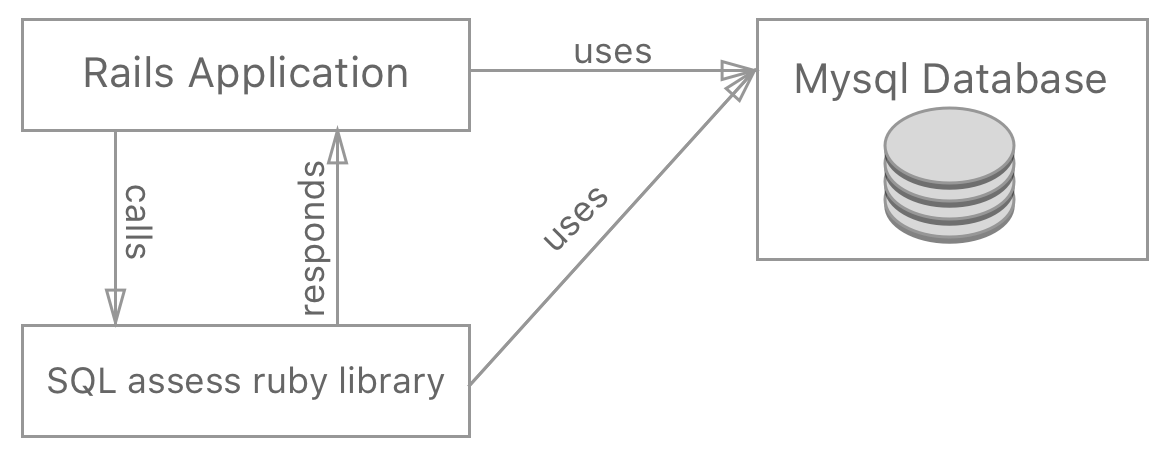
\includegraphics[width=100mm]{images/design/arhitecture.png}
\end{center}

\section{Rails application}
The application will be built on top of $Ruby\ on\ Rails$ (a very opinionated
framework). Rails uses a $Model-View-Controller$ pattern.

\section{SQL grading library}
This Ruby gem will expose a public interface that allows the
comparison of $SQL$ queries and returns a result after comparing the queries.
\begin{enumerate}
    \item $Asessor$ initialized with SQL database information for users. Each user
    will have its own database on the MySQL server.
    \item The schema query (that creates the initial tables and optionally inserts the
    initial data), teacher's query and student's query are passed to the library.
    \item If no data is provided, then the library automatically generates a set
    of data based on the query.
    \item The library creates the tables and inserts the initial data.
    \item The library runs both queries (the student's and teacher's queries)
    and compares the result.
    \begin{itemize}
        \item If the results are the same, then a successful response is sent back
        \item Otherwise, a detailed response with differences is sent back. The process
        for getting the differences is explained in section \ref{design:comparing_the_queries}
    \end{itemize}
    \item All tables and existing data are removed from the database.
\end{enumerate}
\subsection{Comparing the queries} \label{design:comparing_the_queries}
The first process in comparing two queries is canonicalizing the queries.
Those transformations have the purpose of transforming the query clauses in
comparable clauses. For instance, such a transformation transforms a
$BETWEEN$ clause in two $>$ and $<$ queries.
\begin{center}
    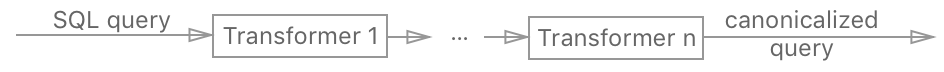
\includegraphics[width=100mm]{images/design/transforming_process.png}
\end{center}
At this point we can then look at each part of the query and see what differences
are: e.g. if there is a missing $WHERE$ clause or if there is a missing column
from the $SELECT$ clause.

\section{Testing the application}
The web application and library will have a test suite with built using $RSpec$, $Shoulda\ matchers$
(for unit tests) and $Capybara$ (for the integration tests).
